\documentclass[a4paper,10pt,english]{article}
\usepackage[utf8]{inputenc}
\usepackage[T1]{fontenc}

\usepackage[english]{babel}

\usepackage{xspace}
\usepackage{graphicx,graphics} 
\usepackage{hyperref} 
\usepackage{mathtools, bm}
\usepackage{amssymb, bm}
\usepackage{complexity}
\usepackage{amsthm}
\usepackage{authblk}
\usepackage{color}
\usepackage{amsmath}


\newcommand\pall{\textsc{pall}\xspace}


\newcommand{\todo}[1]{{\color{red} TODO: {#1}}}
\newtheorem{prop}{Proposition}


\graphicspath{{img/}}

%opening
\title{Contention management for Cloud Ran over an optical ring}

\author[1]{Dominique Barth}
\author[2]{Dominique Chiaroni ?}
\author[1]{Ma\"el Guiraud}
\author[1]{Yann Strozecki}
\affil[1]{David Laboratory, UVSQ}
\affil[2]{Nokia Bell Labs France}



\begin{document}

\maketitle


\section{Description of the network, model, problem}

    Our study takes place in the Cloud-RAN context. The purpose is to centralise the calculation units of some antennas, distributed on the field. To each antenna, called RRH (Remote Radio Head), is associated a BBU (BaseBand Unit) in the datacenter.
      The periodic process is the following: each {\bf period $P$}, every RRH (also called antennas) send some datas thought the ring to it's BBU, then, after a computation time in the BBU, this latter answers to the corresponding RRH. 
      The time between the emission of the message by the RRH and the reception of the answers by the same RRH is called {\bf process time} and must not be too large, considering some 5G standards. That is why the message might be as litle buffered as possible into the nodes, in order to decrease the latency, and thus, the process time of the messages.
      In this paper we will consider that all the BBU are grouped in the same node, called {\bf datacenter}, and that the antennas are distributed on the others node of the ring.
      \todo{je pense que ce paragraphe n'est utile que dans le deliverable, sinon je dois mettre l'equivalent dans l'intro}
  
   
  \subsubsection{Network modeling}
  
   In this entire subsection, the ring is in broadcast and select mode with an emission release policy. We first propose an algorithmic model for the ring. In ~\ref{sec:oportmethods}, we study the behavior of the ring with an opportunistic insertion policies, in which the insertion buffer is managed by two different methods. Finally, we propose and study in ~\ref{sec:deterministicalgorithms} some algorithm allowing the C-RAN PDUs to have $0$ sojourn time in the stations, while the BE PDUs are as little buffered as possible.

The model exposed here has already been studied for another particular topology of network and with different problematics from the ones of this paper. One can find in \cite{latency2017} the complexity results on the problem proposed, and some algorithmic solutions to solve it in star networks.

The network is modeled as a directed graph $G=(V,A)$. Each arc  $(u,v)$ in $A$ is labeled by an integer weight $\omega(u,v)$ which represents the time taken by a message to go from $u$ to $v$ using this arc. A {\bf route} $r$ in $G$ is a directed path, that is, a sequence of adjacent vertices $u_0, \ldots , u_{k}$, with $(u_i,u_{i+1}) \in A$.  The {\bf latency} of a vertex $u_i$ in a path $r$ is defined by $\lambda(u_i,r)= \sum\limits_{0 \leq j <i} \omega(u_j, u_{j+1})$. We also define $\lambda(u_0,r)=0$. The length of the route $r$ is defined by $\lambda (r)= \lambda (u_k,r)$.
We denote by $\cal R$ a set of routes, the pair $(G,\cal R)$ is called a {\bf routed network} and represents our telecommunication network.

   In the context of Cloud-RAN applications, we need to send a message from an RRH $u$ to a BBU $v$ and then 
      we must send the answer from $v$ back to $u$. We denote by $n$ the number of couple RRH-BBU. We say that a routed network $(G, {\cal R})$ is \textbf{symmetric} if the set of routes is partitioned into the sets $F$ of \textbf{forward routes} and $B$ of \textbf{backward routes}. There is a bijection $\rho$ between $F$ and $B$ such that for any forward route $r \in F$ with first vertex $u$ and last vertex $v$, the backward route $\rho(r) \in B$ has first vertex $v$ and last vertex $u$. 
       
 
\paragraph{Messages dynamic}
      
      In the process we study, a message is sent on each route at each period, denoted by $P$. The time is discretized, i.e. a period is sliced into $P$ {\bf slots}. 
      Let $r$ be a route, if a message is sent at time $m$ from $s$ the first vertex of $r$ then it will arrive at vertex $v$ in $r$ at time $m + \lambda(v,r)$. Since the process is periodic, if the message from $r$ goes through an arc at time $t\in [0,P-1]$, then it goes through the same arc at time $t+kP$ for all positive integers $k$. Therefore, every time value can be computed modulo $P$ and we say that the first time slot at which a message sent at time $m$ on $r$ reaches a vertex $v$ in $r$ is $t(v,r) = m + \lambda(v,r)\mod P$. 
      
 A message usually cannot be transported in a single time slot. Let us call $[t(v,r)]_{P}$ the set of time slots used by route $r$ at vertex $v$ in a period $P$, that is $[t(v,r)]_{P} = t(v,r)  \mod P $. Let $r_1$ and $r_2$ be two routes, on which messages are sent at time $m_1$ and $m_2$ in their first vertex.
      We say that the two routes have a {\bf collision} if they share an arc $(v,w)$ and $[t(v,r_{1})]_{P} \cap [t(v,r_{2})]_{P} \neq \emptyset$.
      
         A {\bf $P$-periodic assignment} of a routed network $(G,\cal R)$ is a function that associates to each route 
         $r \in \cal R$ its \textbf{offset} $m_r$ that is the time at which a message is emitted at the first vertex of the route $r$.  In a $P$-periodic assignment, \emph{no pair of routes has a collision}.
                     
                     Let us give an interpretation of a $P$-periodic assignment of $(G,{\cal R})$ a symmetric routed network, so that it represents the sending of a message and of its answer.
	First a message is sent at $u$, through the route $r \in F$, at time $m_r$.
      This message is received by $v$, i.e., the last vertex of $r$ at time $t(v,r)$. It is then sent back to $u$ on the route $\rho(r)$ in the same period at time $m_{\rho(r)}$ if $m_{\rho(r)} > t(v,r)$, otherwise at time $m_{\rho(r)}$ in the next period. The time between the arrival of the message and the time it is sent back is called the \textbf{waiting time} and is defined by $w_r = m_{\rho(r)} - t(v,r)$ if $m_{\rho(r)} > t(v,r)$ and $w_r = m_{\rho(r)} + P - t(v,r)$ otherwise.
      \begin{figure}[h]
      \begin{center}
      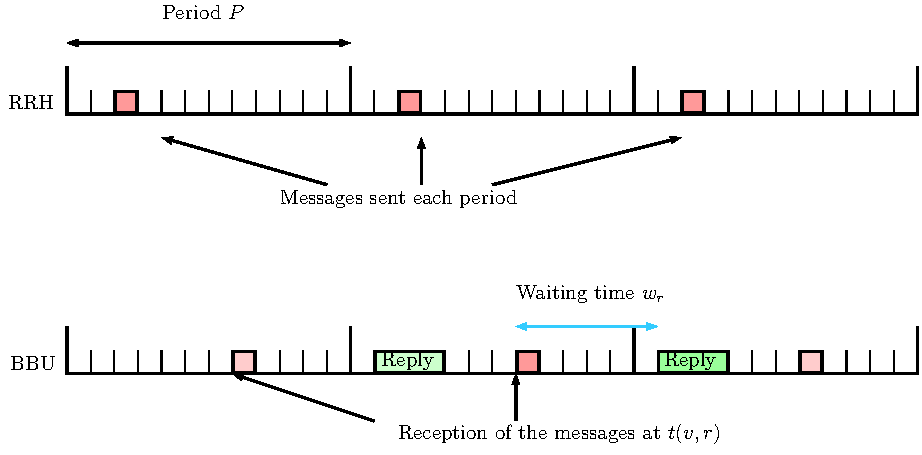
\includegraphics[width=0.9\textwidth]{rrh.pdf}
      \end{center}
      \caption{The process defined by a $P$-periodic assignment}
      \end{figure}

The process time for a message sent on the route $r$ is equal to $PT(r)=\lambda(r)+ w_r+\lambda(r)$. Each route must respect some time limit that we call a \emph{deadline}. To represent these deadlines, 
      we use a deadline function $d$, which maps to each route $r$ an integer such that $PT(r)$ must be less than $d(r)$.
    We can now define a first problem:

      \noindent {\bf Periodic Assignment for Low Latency (\pall)} 

 
      \noindent {\bf Input:}  A symmetric routed network $(G,{\cal R})$, the integers $P$ and a deadline function $d$.
      
      \noindent {\bf Question:} does there exist a $P$-periodic assignment $m$ of $(G,{\cal R})$ such that for all $r \in {\cal R}$, $PT(r) \leq d(r)$?

It turns out that the problem \pall is $\NP$-hard to solve and even to approximate for \emph{general} routed networks, and for the simplified version presented here~\cite{latency2017}.      
          
  \paragraph{N-GREEN Optical ring}
   
 We now consider $G$ as a circular digraph $C_N$ representing an unidirectional optical ring. The vertices of the graph represents the nodes of the ring. In our study, we want to focus on the ring only. Thus, we ignore the external network and we consider that, the first and last vertex , $u$ and $v$ of the routes are some nodes of the ring. We consider a symmetric routed network. For each forward route $r$, the backward route $\rho(r)$ is the other part of the ring. Consequently, for each route $r$, $\lambda(r) + \lambda(\rho(r)) = RS$, where $RS$ is the size of the ring. In our experiments, we consider only one datacenter into the ring. This mean that all the forward routes have the same destination nodes, and all the backward routes have the same source node.

  % Once a packet is inserted in a slot on the ring, by a node, no other nodes are able to write on this slot. This packets can contain some data from several nodes on the ring, that are able to read in the packet. The only node which has the right to remove the packet from the slot is the owner. This mean that every packet makes exactly one lap of the ring. Furthermore, to write on a slot, a node has to have an empty slot in it's writing slot.
% \subsection{Message Granularity}
% Each arc $(u,v)$ can be represented as a sequence of slots $\{s_1, ... , s_k\}$, with $k = \omega(u,v)$. We denote by $s_n(u,v)$ the $n^{th}$ slot of the arc $(u,v)$. $s_i(v), i\in \{-\omega(u,v), ... , -1\} \cup \{1 , ... , \omega(v,w)\}$ is the $i^{th}$ slot after (before if $i<0$) v on the ring.
%    On the following example, the red slot can be denoted by $s_2(u,v)$, $s_2(u)$ or $s_{-6}(v)$. 
%    \begin{figure}[h]
%    \centering
%      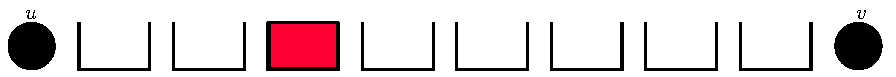
\includegraphics[scale=0.5]{suv.pdf}
%
%      \caption{A link $(u,v)$ represented as a sequence of slots}
%  \end{figure}
%  
%  Each node $v$ has a reading access on $s_{-1}(v)$ and a writing access on $s_{1}(v)$. Those slots are named respectively the reading and writing slots of $v$. Thus, during a time slot, a node $v$ can insert a {\bf container} on it's writing slot, if it is allowed to. At the end of the time slot, each packets rotate to the next slot. A packet emitted by a node $u$ on it's writing slot $s_1(u)$ will be available in reading for a node $v$ on it's reading slot, $s_{-1}(v)$, $d(u,v) -1$  time slots later.
%\begin{figure}[h!]
%      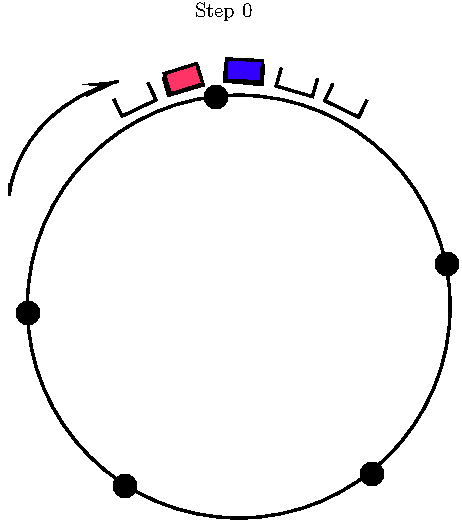
\includegraphics[scale=0.5]{anneau1.pdf}
%      \hspace{3cm}
%      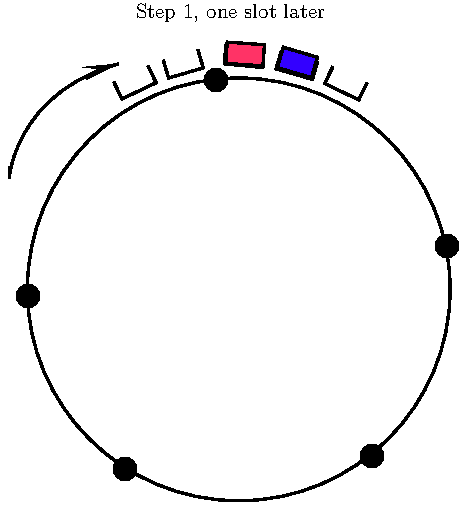
\includegraphics[scale=0.5]{anneau2.pdf}
%      \caption{One rotation of the ring}
%  \end{figure}

\paragraph{Into the node : Two kind of traffics}
  In this study, we focus on the behavior of the N-GREEN optical ring. Therefore, we do not want to consider the issues caused by the upstream network. 
   To refine our model around the N-GREEN study, one must consider the opto-electronic stations behavior.
   Each N-GREEN station is connected to at least one electronic interface of rate $D$. as mentioned in sec.\ref{com-mod} a station is able to use all the $K$ channels during a slot of duration $Z/KD$ to send a container of capacity $Z$ which contain all the data received  by an electronic interface during a macro-slot, that is, the time needed to fill a container at rate $D$, i.e. $Z/D$
  In other words, an N-GREEN station is able to fill a PDU with the datas received during a macro-slot in the electronic domain. 
    
\begin{figure}[h!]
\begin{center}   

      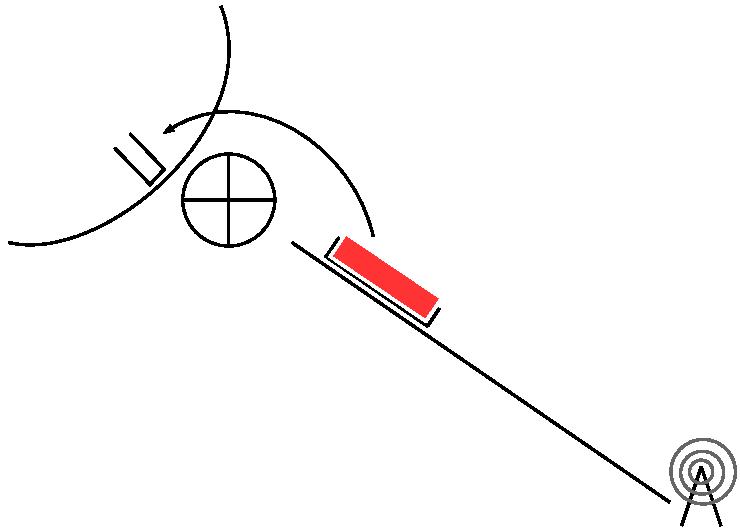
\includegraphics[scale=0.3]{slot1.pdf}
  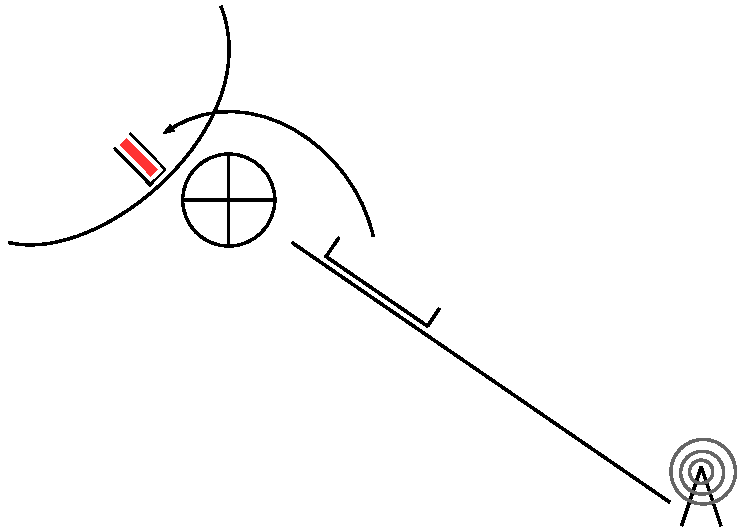
\includegraphics[scale=0.3]{slot2.pdf}
     \caption{Opto-electronic interface.}
     
\end{center}
  \end{figure}
  
  
      An N-GREEN station deals with two kinds of traffics. Some C-RAN and some Best Effort. We assume that each traffic has its corresponding electronic interface. Also, a C-RAN message is of size $Z $ and completely fills a container let us call {\bf C-RAN PDU} such a message. In the same time, the Best Effort SDUs are buffered in a first {\em gathering buffer} before being gathered together into a {\bf BE PDU}. Once the PDUs are created, there join the {\em contention buffer} before being sent in the ring.
      \begin{figure}[h!]
\begin{center}   
  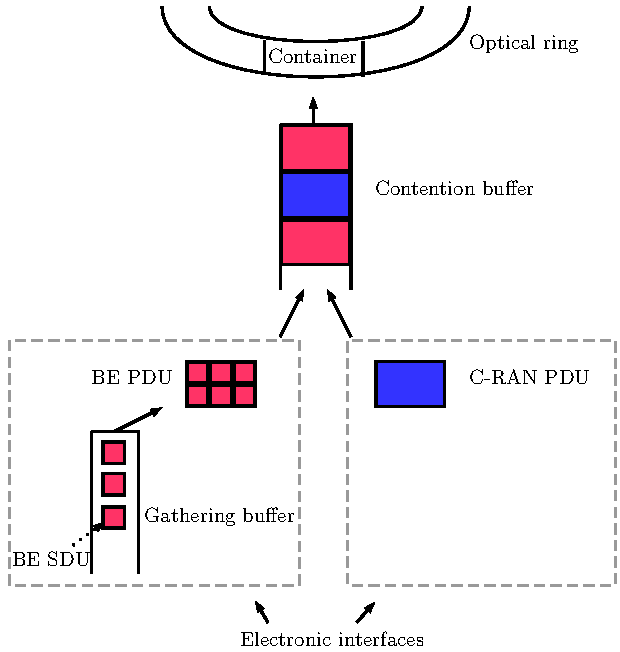
\includegraphics[scale=0.7]{buffers.pdf}
     \caption{An N-GREEN station.}
     
\end{center}
  \end{figure}
  
 In this study, we measure the sojourn time $W$ of a PDU in a station. The model we consider in our experiments to generate the BE PDUs is described in sec~\ref{jmf}.
  
 \paragraph{C-RAN PDU generation model} An RRH usually emit an huge quantity of information during a long time. Also, as we just see, an RRH can send no more than a PDU every $10\mu s$ on the ring. This gap between two PDU from the same RRH is defined by $K$, the number of channels considered in the ring.
 We denote by $ET$,for {\bf Emission time}, the time during which an RRH emits a PDU every $K$ slots on the ring. An RRH emits $\frac{ET}{K}$ PDUs on the ring, every period $P$.
    	    
        \begin{figure}[h!]
\begin{center}   

      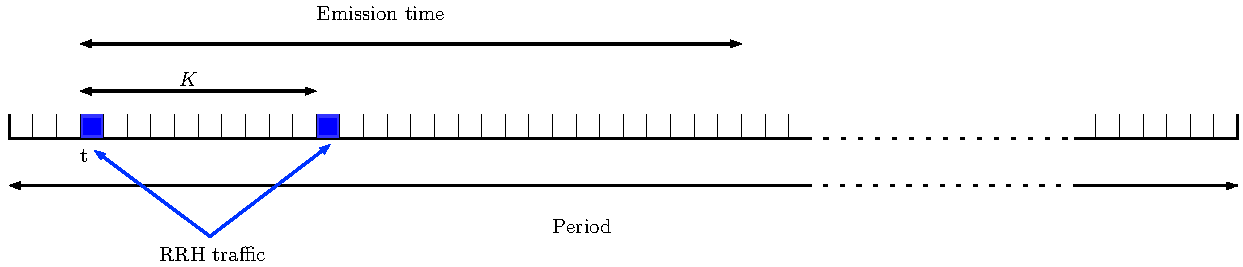
\includegraphics[width=\textwidth]{emission_antenna.pdf}
     \caption{C-RAN PDU generation.}
\end{center}
  \end{figure}
  \paragraph{Back and forth communications} As we explained in the introduction of this section, once the datacenter receives some PDUs from an RRH, it computes an answer and send it to the RRH through the ring. To simplify our model, we assume that the computation times is the same for all BBUs and that it is a multiple of the period. In this situation, we can assume that, each time the datacenter receives a container with a C-RAN PDU from an RRH, it immediately sends an answer (which is in fact the answer to the two periods ago C-RAN PDU's).
  
  
 The behavior of the C-RAN PDU generation leads us a new problem, similar to \pall. The set of time slots used by route $r$ at vertex $v$ in a period $P$, is now defined by $[t(v,r)]_{P,K} = \{t(v,r) +i \mod P \mid i \in \{0,EP,2\times K,...., \frac{ET}{K}\times K\} \}$. Consequently, we now want to find a $(P,ET)$-periodic assignment that set the offsets of the routes $m_r$, such that there is no collision between two routes $r_1$ and $r_2$, that is, $[t(v,r_{1})]_{P,K} \cap [t(v,r_{2})]_{P,K} \neq \emptyset$. 
  
  
  
 The rest of this study is divided in two parts. In a first time, we look at the behavior of the ring and the impact of the PDUs sojourn time with two different method of managing the contention buffer. Then, we propose some algorithms that solve the previous problem of finding a $(P,ET)$-periodic assignment for the C-RAN PDUs and we compare the impact of those different algorithms on the BE PDUs sojourn time.

  \paragraph{Parameters of the study}
  \label{sec:parameters} The experiment of this subsections are made following the same parameters, until sec~\ref{sec:optialgo}. We set $K = 10$ chanels, some electronic interface of rate $D=10$Gbps and $Z = 12500$B so, $Z/KD = 1\mu$s. The optical ring has a rate $KD=100$Gbps, while a slots has a duration of $1\mu$s. The length of the ring is to $20$km in our simulations, this means that the ring has a length of $RS = 100$ slots. We consider some BE SDUs of $125$B, and we parametrized BE PDU generator of sec~\ref{jmf} such that each station load the network with an average of $3,5\%$ of BE traffic. We set $ET = 500$ slots, that correspond to a C-RAN traffic of $5$Gbps. The period  $P$ is to $1$ms, that is $1000$ slots. We set the number of RRH to $n=5$. We take $5$ stations and one of them is the datacenter. The antennas are apportioned between the others station. With those parameters, the network is theoretically loaded to $67.5\%$. 
  
  \begin{figure}
  \centering
  \begin{tabular}{|c|c|}
  \hline
 Number of channels $K$ & $10$  \tabularnewline
  \hline
  Rate of an electronic interface $D$ & $10$ Gbps \tabularnewline
  \hline
  Container size  $Z$ & $12,500$ B  \tabularnewline
  \hline
  Slot duration $Z/KD$ & $1\mu$s \tabularnewline
  \hline
  Optical ring rate $KD$ & $100$ Gbps \tabularnewline
  \hline
  Length of the ring $RS$ & $100$ slots \tabularnewline
  \hline
  BE SDU size & $125$B \tabularnewline
  \hline
  C-RAN PDU size & $12,500$B$=Z$ \tabularnewline
  \hline
  Emission time $ET$ & $500$ slots \tabularnewline
  \hline
   Period $P$ & $1,000$ slots \tabularnewline
  \hline
  Number of RRH & $5$  \tabularnewline
  \hline
  Number of stations $n$ & $5$  \tabularnewline
  \hline
  
  \end{tabular}
  \caption{Parameters of the following experiments based on N-GREEN}\label{parameters}
  \end{figure}
  
   \subsubsection{Performance evaluation of the N-GREEN optical ring}
   \label{sec:oportmethods}
   In a first time, we will look at the performance of the N-GREEN optical ring with an opportunistic insertion policy \ref{com-mod}. When a station wants to send a PDU on the ring, it uses the first available container .
    We study the performance of the ring through two methods; a full opportunistic method, and a method that prioritize the C-RAN PDUs. Since we only consider some PDUs arrivals, those two methods are some variants of the management of the PDUs in the station.
   For those two methods, the offsets $m_r$ of the routes are chosen randomly in the period, i.e. we do not choose the first time at which the RRH start to emit.
   Since we do not manage those offsets, the two following methods do not gives us some $(P-ET)$-periodic assignment. No choices are made on the offsets and thus, two routes can collides. 

    
    \paragraph{Full opportunistic method}
    \label{sec:fullopport}
    We first want to look at a simple configuration in which we do not manage the PUDs (BE or C-RAN) arriving into a station. At their arrival, the BE and C-RAN PDUS are buffered in the contention buffer, and this buffer is emptied following the FIFO rule.

The following experiment shows us the performance this {\bf full opportunistic method} with some parameters issued from N-GREEN. 
On fig~\ref{fig:oport}, one can see the cumulative distribution of the sojourn times of the C-RAN and BE PDUs. Those results are computed on $100$ instances of optical rings that have run during $10,000,000$ slots. The measures are taken after $3,000$ slots of simulation, to let the ring initialize it's behavior. The parameters of the simulations are stated in sec~\ref{sec:parameters}.


    \begin{figure}[h!]
    \label{fig:oport}
        \begin{center}
      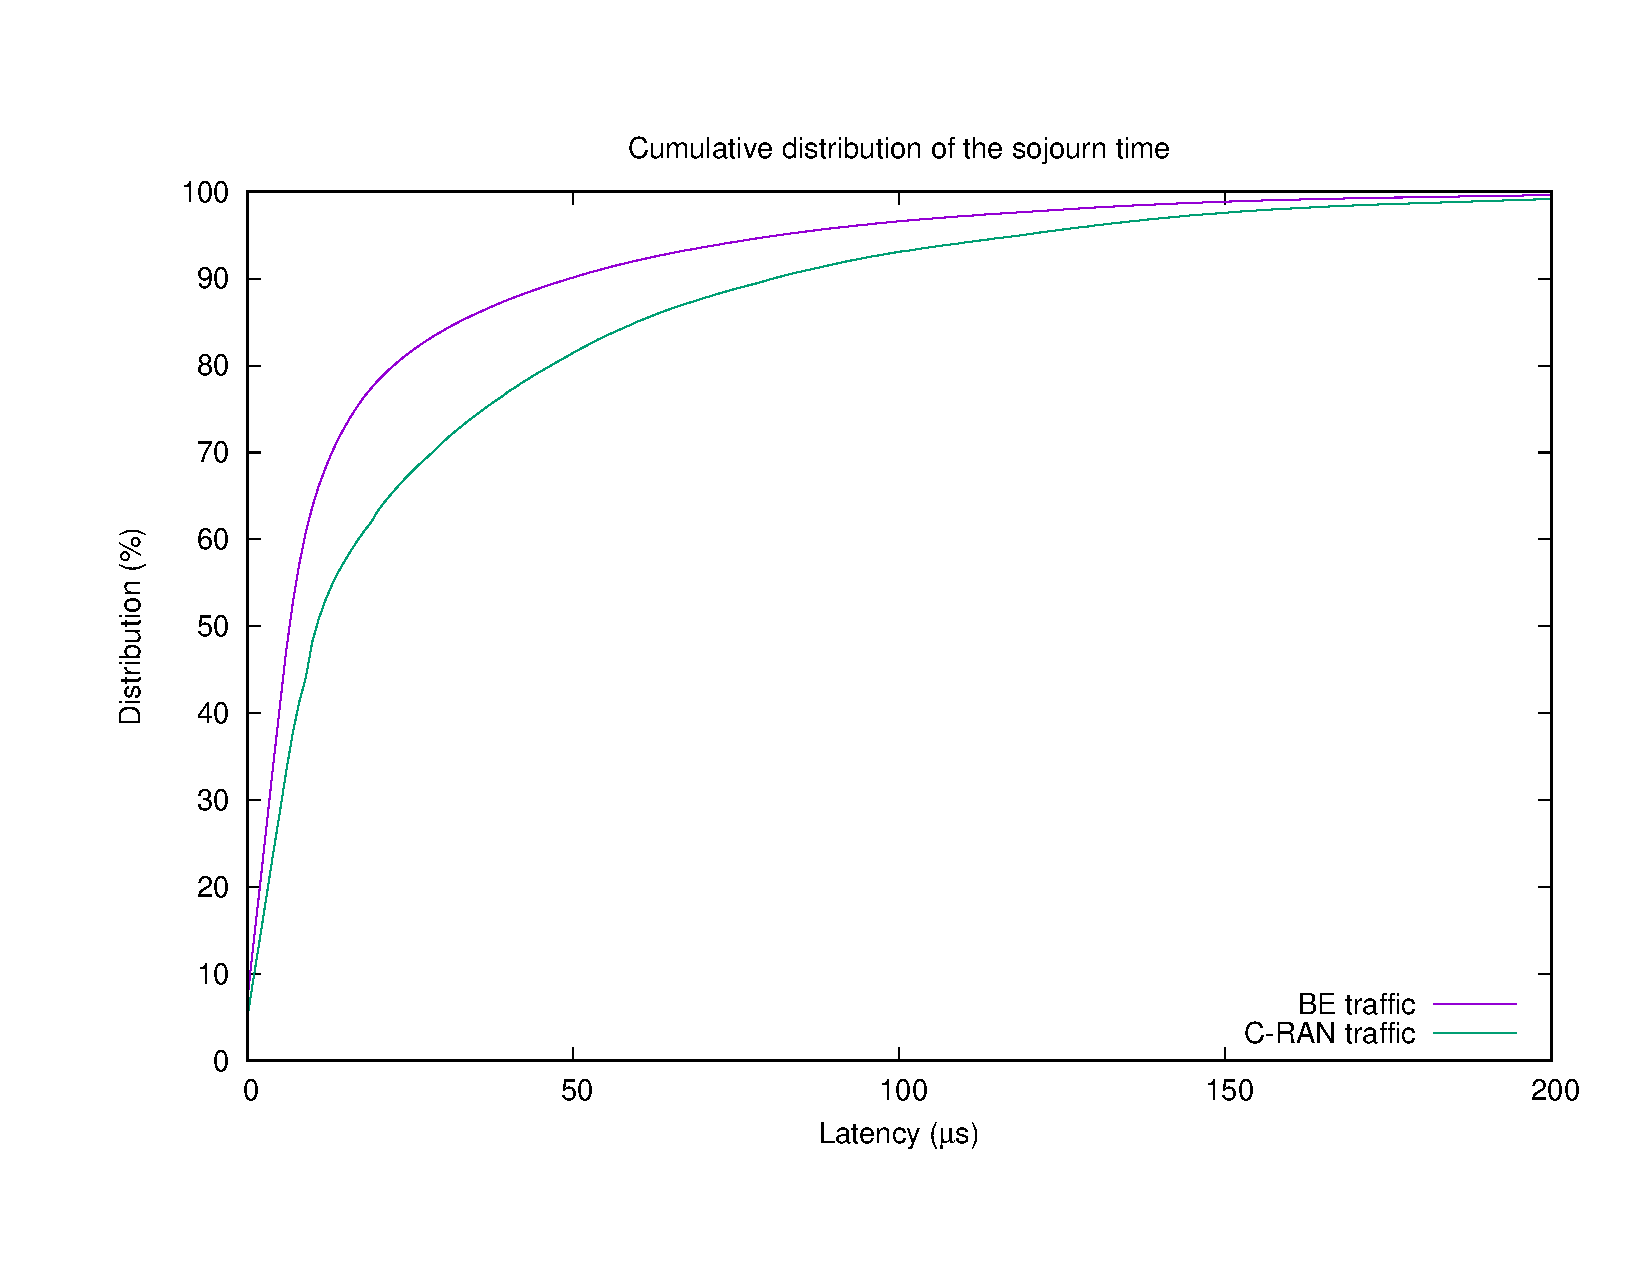
\includegraphics[scale=0.4]{oport}

      \caption{Full opportunistic method performances.}
      \end{center}
  \end{figure}
  
  As we can see on fig~\ref{fig:oport}, the sojourn times for the different kind of PDU is notably similar because we do not manage anything. Furthermore, we can remark that about $10\%$ of the C-RAN messages wait over $100$ms, that is already critical for C-RAN \todo{ref}.

\paragraph{C-RAN priority method}
\label{sec:cranprio}
  In order to improve the C-RAN PDUs sojourn time, we imagined the following solution, called {\bf C-RAN priority method}. Each stations have two contention buffers. One for the BE PDUs, and one fore the C-RAN PDUs. When a station is able to send a PDU on the ring, i.e. its available container free, the container is filled with the C-RAN PDUs first. 
  
    \begin{figure}[h]
\begin{center}   
      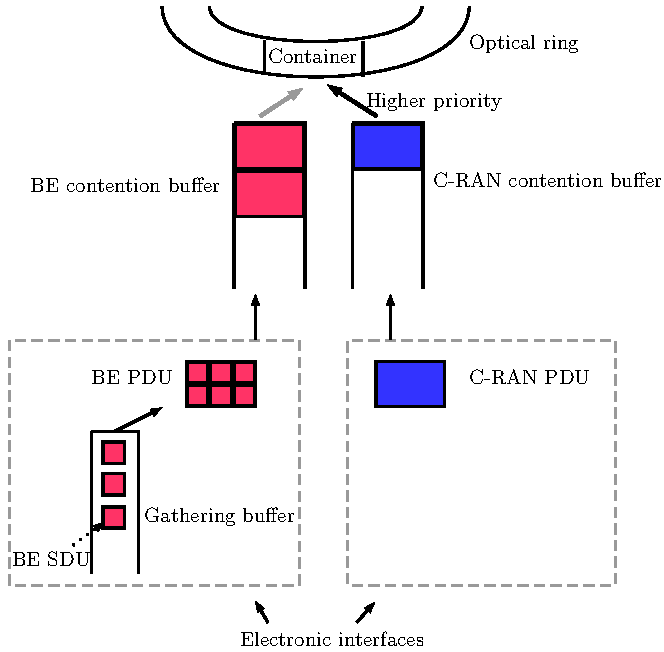
\includegraphics[scale=0.7]{cranprio.pdf}
     \caption{C-RAN priority method.}
\end{center}
  \end{figure}
  
  With this method, one can imagine improve the sojour time of the C-RAN PDUs. Fig~\ref{fig:prior} shows us the performance of the C-RAN priority algorithm for different kinds of traffics. The parameters of the simulations still the same, stated in sec~\ref{sec:parameters}.
      \begin{figure}[h]
      \label{fig:prior}
\begin{center}   

      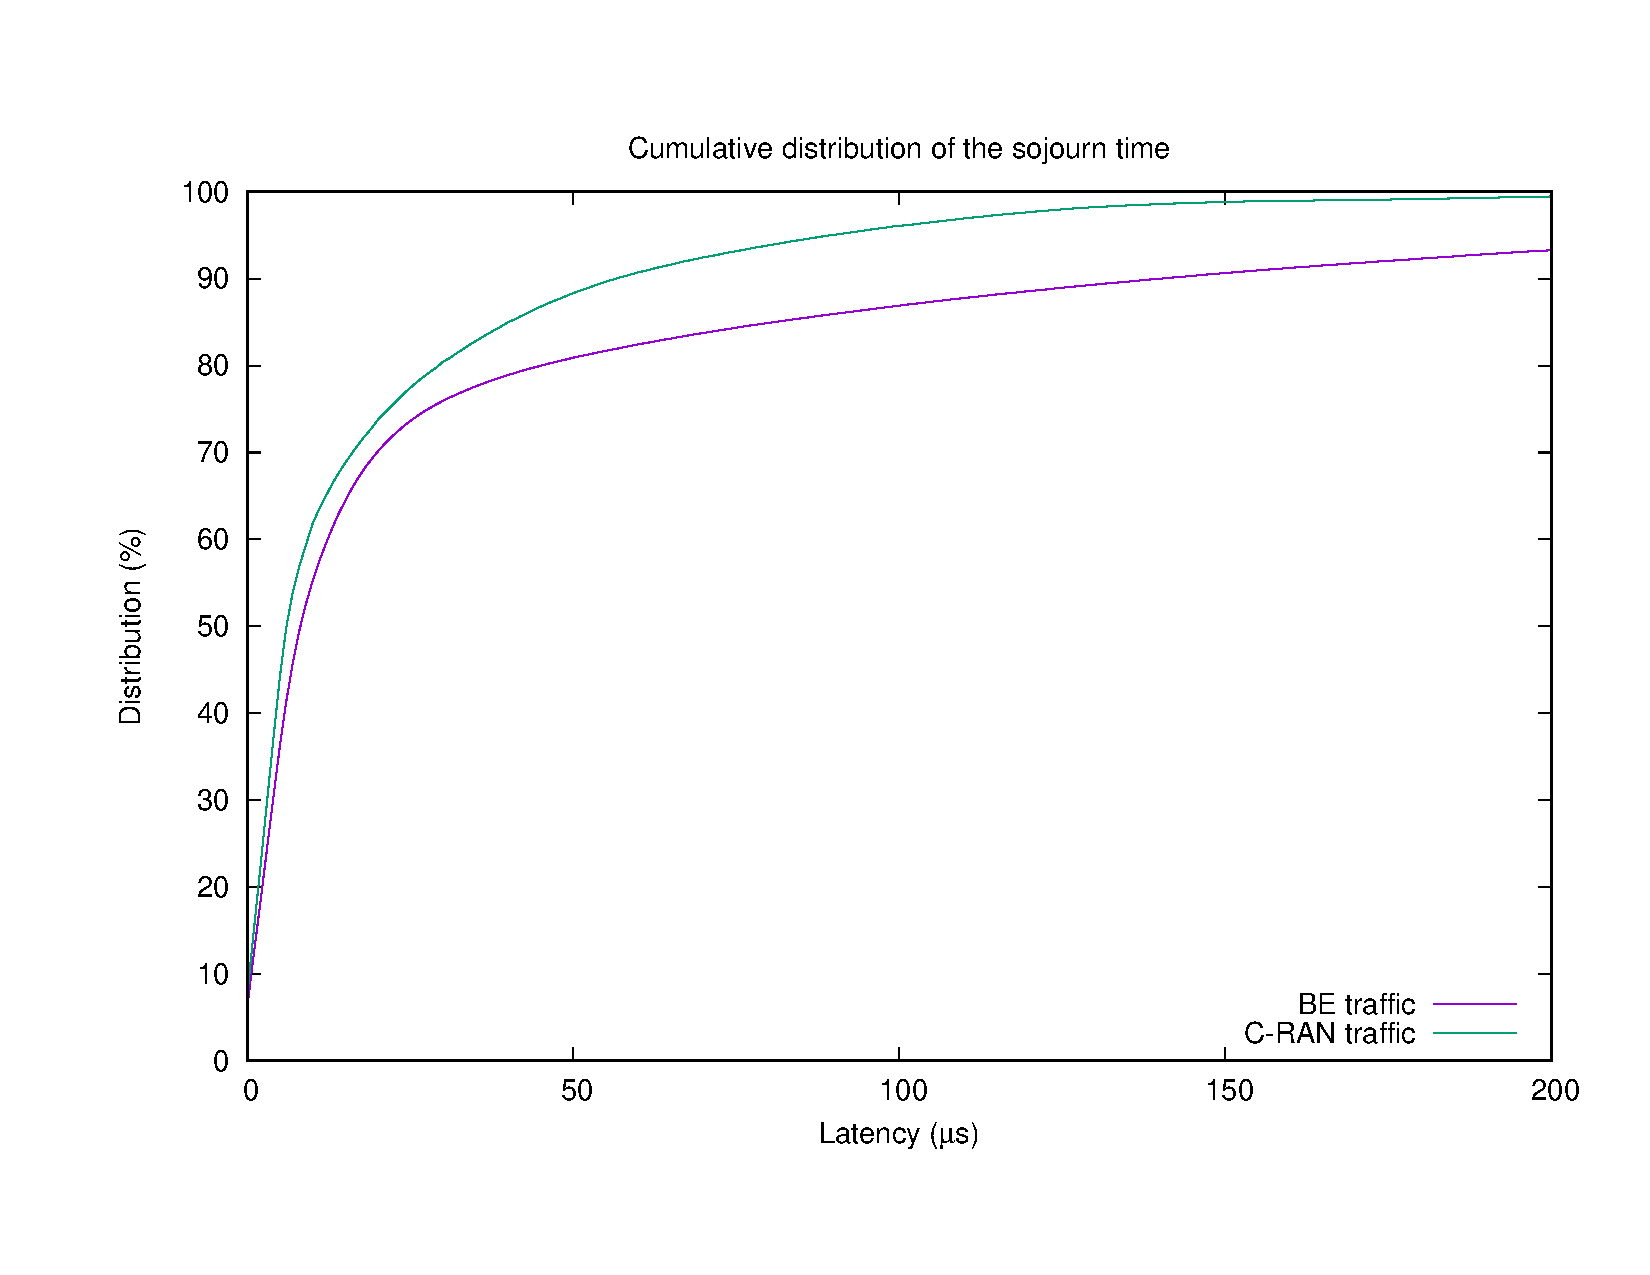
\includegraphics[scale=0.4]{prior.pdf}

     \caption{C-RAN priority method performances.}
\end{center}
  \end{figure}
  
  As expected, the sojourn time of the C-RAN PDUs is decreased compared to the full opportunistic method. Nevertheless, there is still $10\%$ of the C-RAN PDUs that have more than $50 \mu$s of latency, and the best effort PDUs are penalized, indeed, close to $10\%$ of the BE PDUs awaits more than $150\mu$s before being sent in the ring, versus close to $0\%$ with the previous method..
  Thus, we propose a deterministic approach in which we set the offsets of the RRH and we reserve the containers needed for the C-RAN PDUs.
   \todo{il manque une partie sur le travail de karim, }
  \subsubsection{Deterministic approach for $0$ sojourn time on C-RAN}
\label{sec:deterministicalgorithms}

 For the rest of the subsection, the policy of slot insertion is the slot reservation. We are still in emission release policy. We present three algorithms that allows the C-RAN PDUs to have $0$ sojourn time in the insertion buffers by establishing a static reservation of the slots in the period.
 Those algorithm are {\bf Centralized} and requires a global supervisor of the network to be implemented .\todo{phrase + ref sdn?}
 
\paragraph{Slot reservation} To decrease the C-RAN messages sojourn time, one plan to reserve the container for the stations. Indeed, if a station $i$ needs to send a PDU at time $t$, a container needs to be reserved since the previous lap of the container, i.e. at time $t - RS$ by $i$. In this situation, if the container is already taken by a PDU which has been sent by a station $j$, $j$ will remove the PDU of the container during the next lap of the ring, and no other stations are able to write in this container before it comes back to the station $i$ a date $t$. By finding a $(P,ET)$-periodic assignment and reserving the corresponding container, we allow the C-RAN PDUs to have $0$ sojourn time in the stations. Though, it impacts the best effort PDUs, by avoiding them to use free reserved containers. It is equivalent to increase the load of the network, without increasing the number of PDUs carried by the network. 

\paragraph{RRHs synchronisations}
This slot reservation implies that the RRHs are synchronized with the ring. The following proposed algorithms set a sequence of reserved slots for each RRH in each period. A technical application implies to simultaneously ensure the reservation of the slot to the given dates, and the synchronization of the RRH with those reserved slot. One must ensure that the C-RAN PDU arrives in the contention buffer of the station just before the reserved container.

In this section, we explain the different algorithm we use to ensure $0$ sojourn time on C-RAN PDUs and we study their impact on the BE PDUs sojourn times.
  
Unlike the previous methods with opportunistic insertion policy, we now want to choose a $(P,ET)$-periodic assignment for the routed network $(G,{\cal R})$. Since all the forward routes have the same last vertex $v$ (the datacenter), which is also the first vertex of all the backward routes, we choose to manage the collision in this vertex only. The purpose is to determine the time $t(v,r_i)$ at which the first C-RAN PDU of the route $i$ arrives at the datacenter $v$ for each routes $i$, such that there is no collisions between the routes. Let us call BBU-offset this time. Once the BBU-offsets are set, for all routes $i$, it is easy to compute $m_{r_i} = t(v,r_i) - \lambda(v,r_i)$.


\paragraph{An approach based on N-GREEN parameters}
An RRH can not emit a message more often than once slot every $K$ slots. Remember that {\bf macro slot} is a duration of $K$ slots, during which each RRH can emit at most once. Thus, we consider the simple case in which there is less C-RAN traffic than slots in a macro slot. Indeed, in that case, if we manage the collision in one macro slot, i.e. we assign a C-RAN traffic to each slot of the macro-slot, we find a  $(P,ET)$-periodic assignment. Since a BBU always instantly emits an answer to it's RRH, for each RRH, a group of two following containers (called {\bf bunch}) can be reserved. Thus, we first study the case $K \ge 2\times n$. As a reminder, $n$ is the number of couple BBU-RRH. 

 
 Because there is at most as much couples BBU-RRH as bunches, we want to assign one RRH to one bunch.
We propose the following {\bf naive reservation algorithm}. For each RRH $i, i\in \{0,...,n-1\} $, set $t(v,r_i)= 2\times i$ with $v$ the vertex of the BBUs. The model automatically fixes the offset of the backward route $\rho(r_i)$ to $m_{\rho(r_i)}= 2\times i +1$. This is the reason why we do not care about the backward routes anymore, and we only deal with the BBU-offsets of the forward routes..
   \begin{figure}[h]

      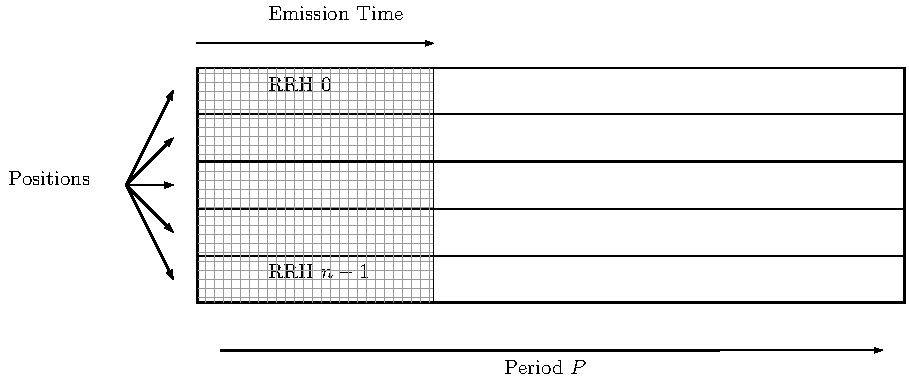
\includegraphics[scale=0.7]{freqgrouped.pdf}
     \caption{Grouped assignment of the bunches to the RRH.}   \label{fig:freqG}
  \end{figure}


We kept the same parameters than in the two previous experiments (see~\ref{sec:parameters}) and we made an experiment to show the impact of this algorithm on the BE traffic. Fig~\ref{fig:res1} shows us the distribution of the sojourn time for BE PDUs with this algorithm.

      \begin{figure}[h]
\centering
      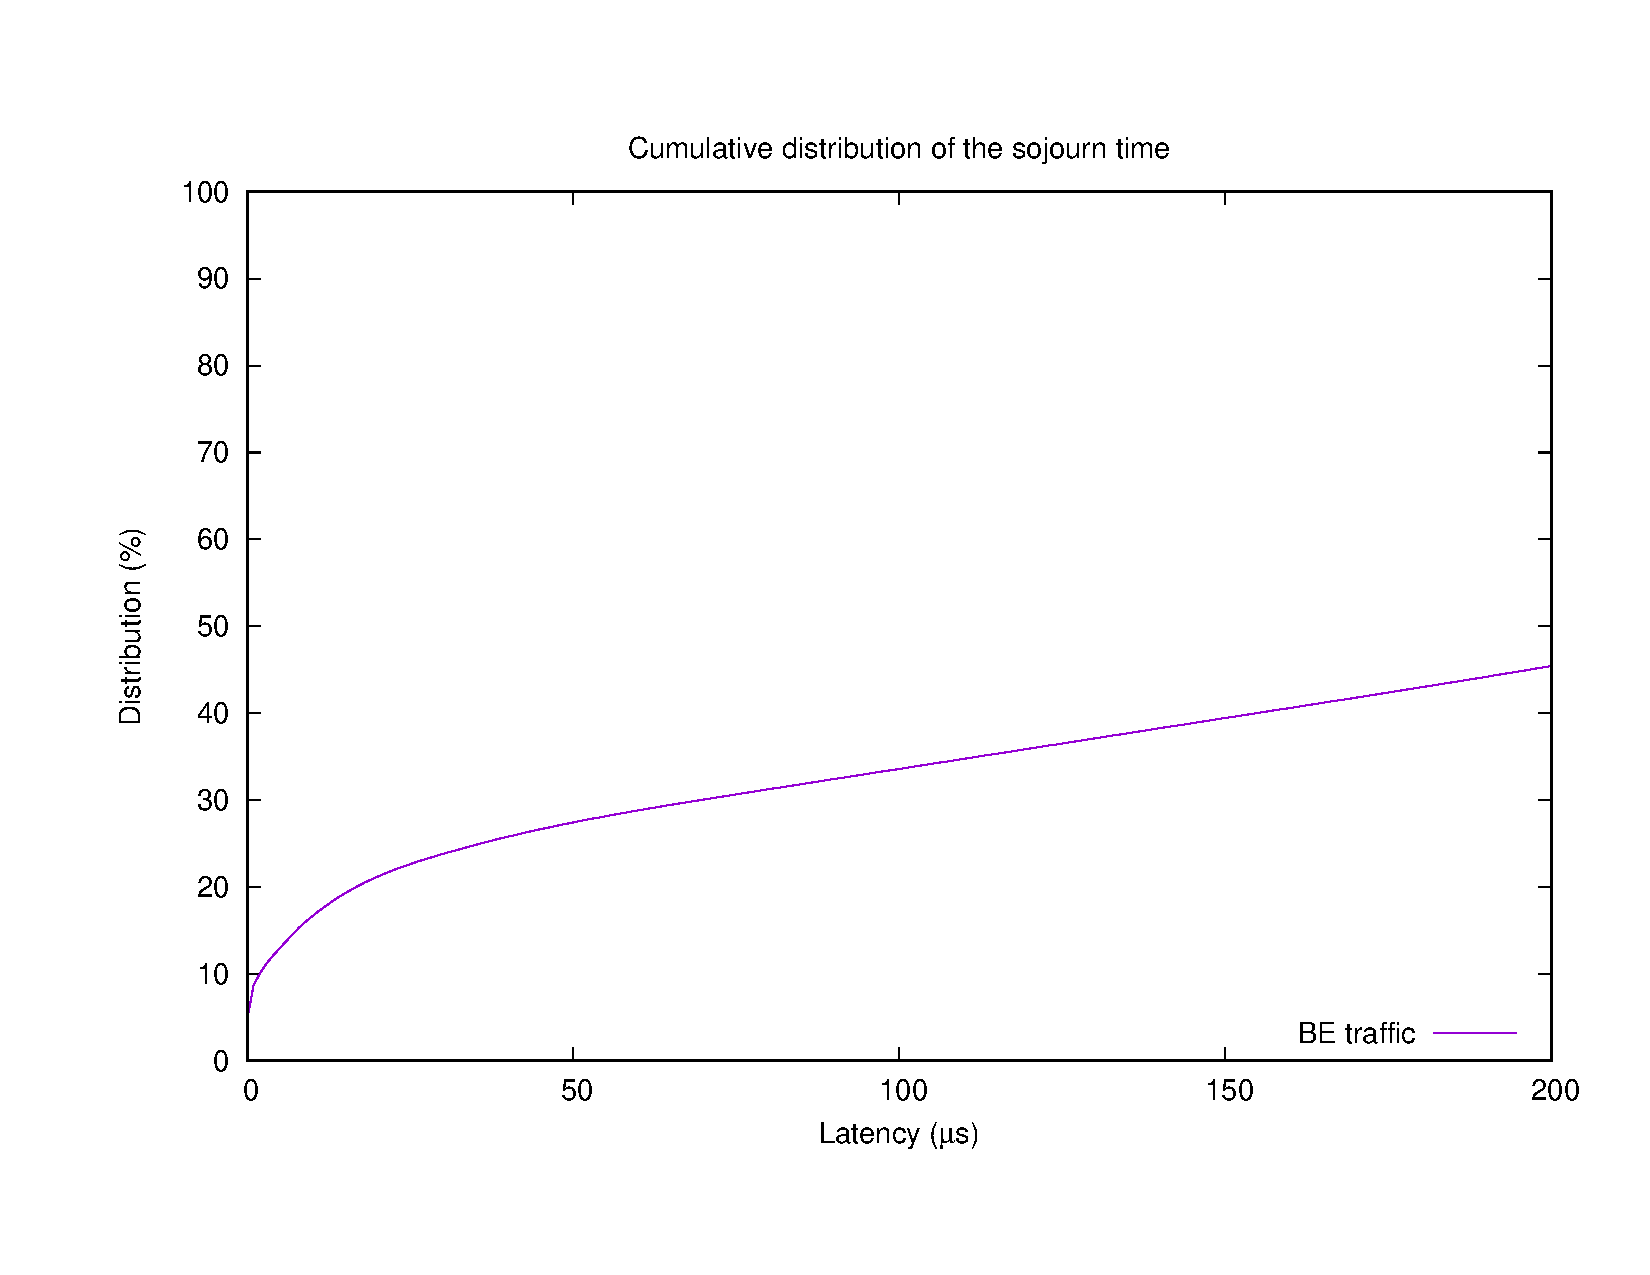
\includegraphics[scale=0.4]{res1.pdf}
     \caption{Impact of the naive reservation algorithm on the Best effort PDUs.}   \label{fig:res1}
  \end{figure}

As we can see, the BE traffic is highly penalized by this algorithm, indeed, while almost $100\%$ of the BE PDUs have a sojourn time to less than $200 \mu$s with the full opportunistic method (see fig~\ref{fig:oport}), here, more than half of the BE PDUs are be buffered more than $200\mu s$. Those performances are explained by the structure of the algorithm. The messages are grouped together, and with our parameters, $K = 2\times n$. It creates a long sequence of slots during which there is no free containers in the ring. 

To improve the BE PDUs sojourn time, we propose a {\bf splited reservation algorithm} that balances the load of the CRAN traffic over the period. Instead of giving some close BBU-offsets for all routes $i$, with $v$ the datacenter, we now uniformly distribute the different BBU-offsets in the period. Each couple BBU-RRH is still assigned to its bunch, but we split the BBU-offsets of $\frac{P}{n}$, that is $t(v,r_i)= 2\times i+ i\times \frac{P}{n}$, with $i \in \{0,...,n-1\}$.

   \begin{figure}[!h]

      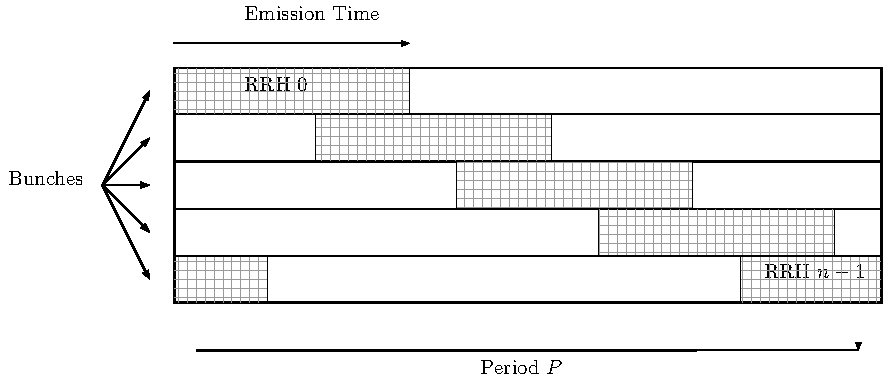
\includegraphics[scale=0.7]{freqsplited.pdf}
     \caption{Splited assignment of the bunches to the RRH.}   \label{fig:freqS}
  \end{figure}
  
  On fig~\ref{fig:res2} one can observe the performance of this algorithm on the BE PDUs sojourn time. Once again, to have a reference point, we take the same parameters for the simulation.

 \begin{figure}[h]
\centering
      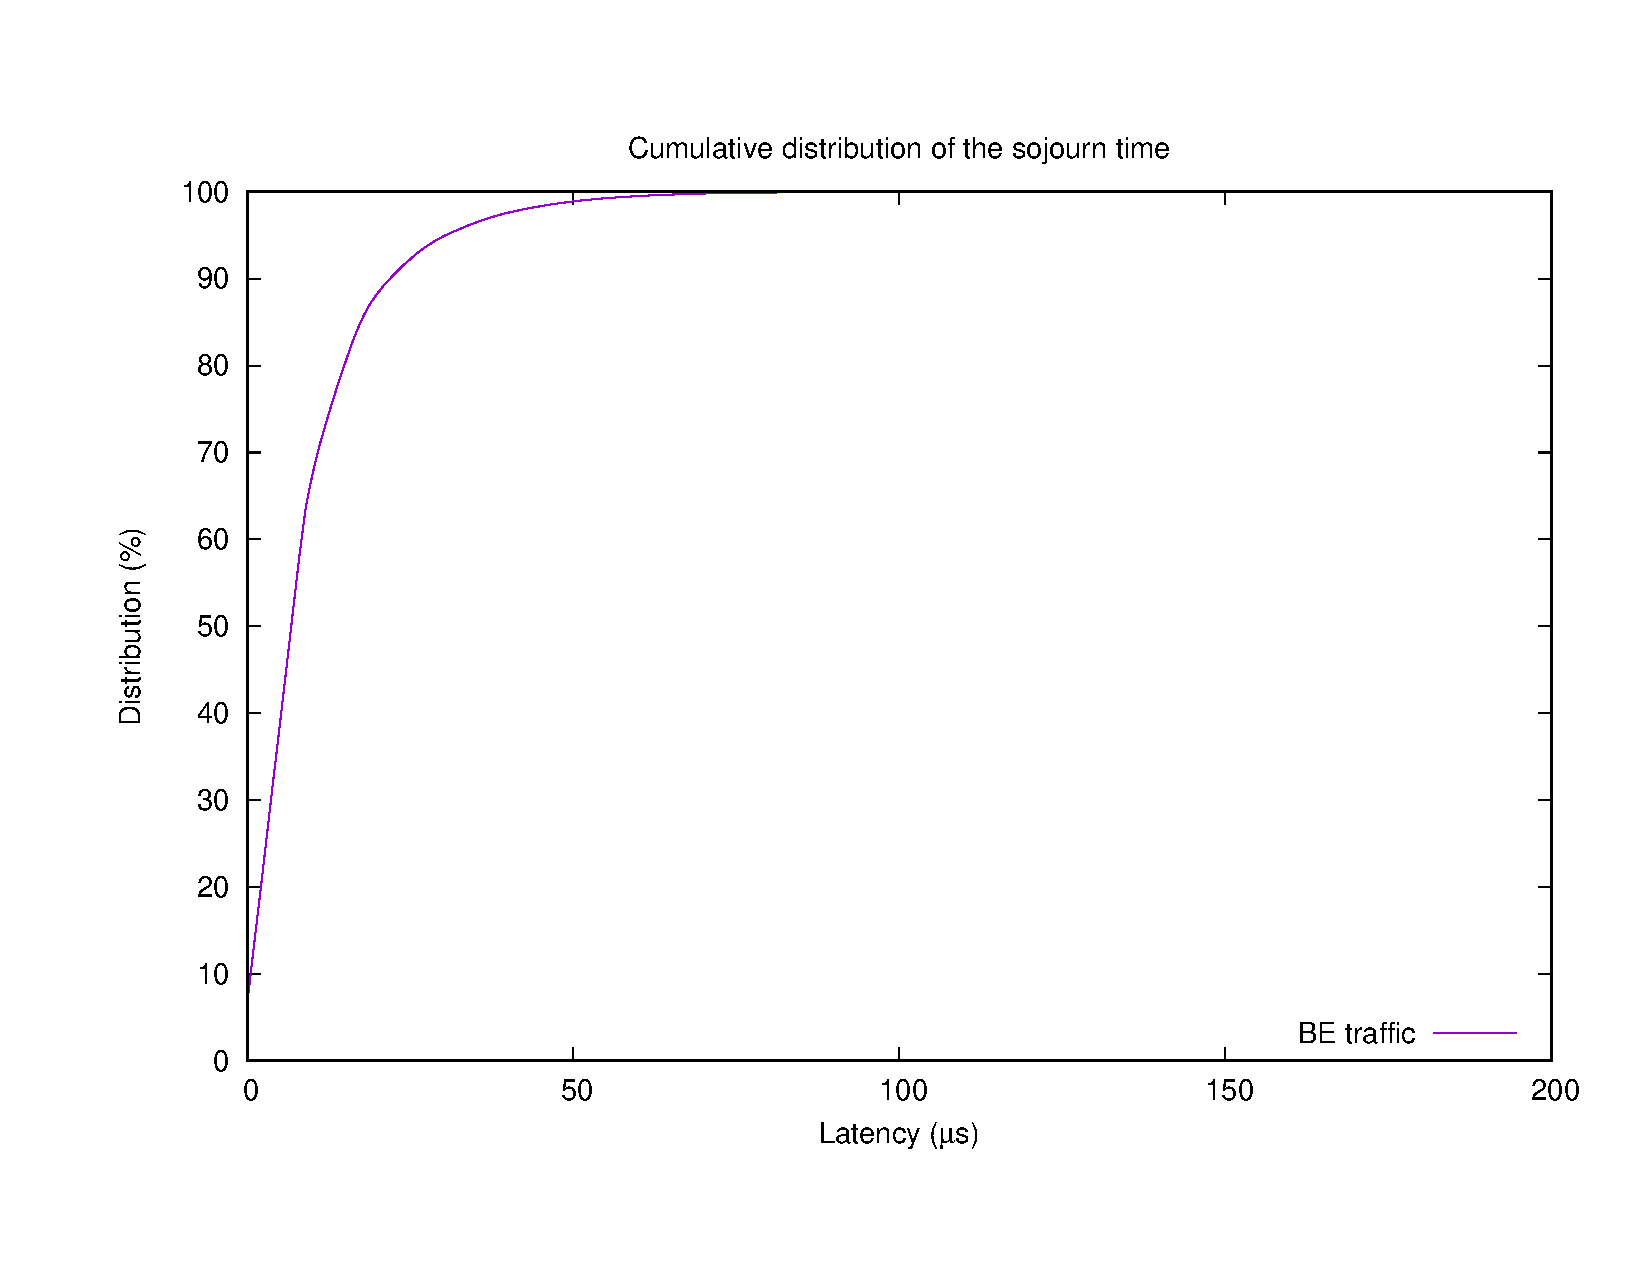
\includegraphics[scale=0.4]{res2.pdf}
     \caption{Impact of the splited reservation algorithm on the Best effort.}   \label{fig:res2}
  \end{figure}
  
  As we can see, the sojourn time of the BE PDUs is highly better with this this algorithm. Indeed almost $100\%$ of CRAN PDUs have a sojourn time of less than $50\mu$s which is better than the full opportunistic method. Thus, we decreased the latency of every kind of traffic.

\paragraph{With more antennas}
\label{sec:optialgo}
 In this section, we study the case $n > \frac{K}{2}$, we want to assign more than one RRH to a bunch. 
 Let us consider a particular behavior of the ring. Instinctively, we can think that if we have enough space in the period for many traffics on the same frequency that is, $ET \le \frac{P}{2}$, we can assign several couples BBU-RRH to the same bunch.

 Let us take $ET =  \frac{P}{2}$ and $n = \frac{K}{2} + 1$. We assign a bunch to each $\frac{K}{2}$ first RRH and we have only one RRH left. Then, we only look at one bunch, on which we want to add the new couple BBU-RRH. 
 
 We take a ring with two stations $A$ and $B$. We simplify the model to only look at the behavior of one bunch, thus, both of the nodes alternatively emits some containers every slots, during $ET$ slots in the period $P$. By construction, we allow $A$ to emit a time $1$ during $ET$ slots. This container arrives in $B$ at $\omega(A,B)$, that is  $[t(B,r_A)]_{P,K} = [\omega(A,B);\omega(A,B)+ET]$. Then, $B$ can immediately emit its containers at time $\omega(A,B)+ET$. This containers from $B$ arrives at $A$ at time $\omega(A,B)+ET + \omega(B,A) = ET + RS$, and thus, $[t(A,r_B)]_{P,K} = [ET + RS;ET + RS + ET] = [ET+RS; RS + P] = [ET + RS; RS] \mod P$. Since $[t(A,r_A)]_{P,K} = [1;ET]$, there is a collision at the interval $[1;RS]$ in the period between the two routes $A$ and $B$.
  \begin{figure}[h]
\centering
      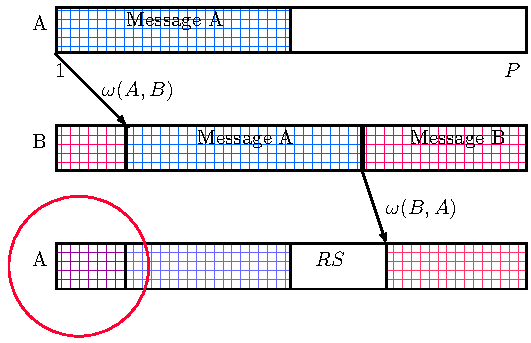
\includegraphics[scale=0.7]{rs.pdf}
     \caption{Collision between two routes on the same bunch when the period is too small.}   \label{fig:proofrs}
  \end{figure}

 
 
 As we have just noted, if several RRH share the same bunch, the period must have an additional budget in addition to the time needed to send the messages. Let us study the size of the additional budget.
 \begin{prop}
 If several RRH shares a bunch, it is possible to find a $(P,ET)$-periodic assignment if $P \ge n\times ET + RS$ , with $n$ the number of RRHs.
 \end{prop}
 \begin{proof}
 We seek to show that proposition by induction.
 
 {\bf Base case:} For $n = 2$, the proof of the previous example shows us that it is possible to assign two RRH on the same bunch with $P = 2\times ET + RS$.
 
 {\bf Induction step:}  We consider that we have a frequency shared by $n$ RRH, with a period of size $P= n\times ET + RS$. We want to show that if we want to add one antenna to the bunch, we need a period of size at least $P = (n+1)\times ET + RS$. If we look at the sequence period of the bunch with $n$ RRH. We can observe that this sequence is the same in every station, shifted of the length of the routes between two stations. For instance, if we take two stations $A$ and $B$, the sequence in $A$ is the same that the sequence in $B$ shifted of $\omega(A,B)$.
 
   \begin{figure}[h]
\centering
      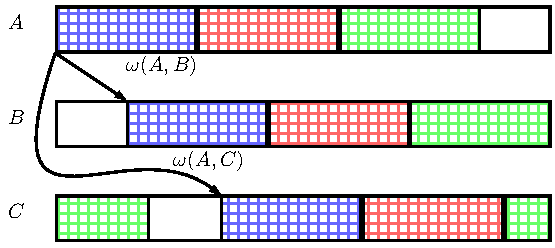
\includegraphics[scale=0.7]{period1.pdf}
     \caption{An example of sequence with n = 3.}   \label{fig:proofperiod1}
  \end{figure}
   
 Thus, if we add $ET$ slots in this frequency, the periodic emissions of all others nodes are not impacted, there is just a new interval in the sequence.
 
   \begin{figure}[h]
\centering
      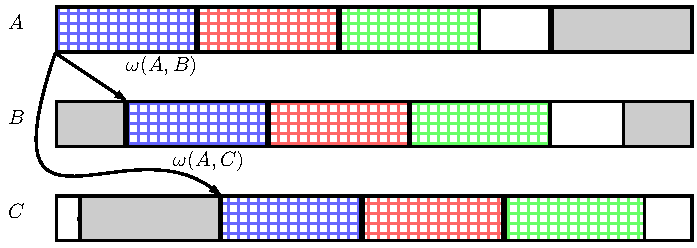
\includegraphics[scale=0.7]{period2.pdf}
     \caption{The same sequence with n = 4.}   \label{fig:proofperiod2}
  \end{figure}
  Note that a station can send some traffic from more than one antenna, the figures ~\ref{fig:proofperiod1} and \~ref{fig:proofperiod2} are just an example, but this proof stays the same.
 \end{proof}
 
Considering those results, we propose an algorithm to allow several RRH to share the same bunch, as long as $P \ge n\times ET + RS$. 
Since we need $RS$ slots on a each bunch with at least an RRH to assign another RRH to this latter, it is interesting to fill as far as possible the bunches. We then compute the number of bunches needed to carry the number of RRH $n$. Then, the algorithms tries to balance those bunches into the macro-slot, i.e. it avoids to group the used bunches together.
The used bunches have $RS$ or more free slots in the period. Thus, the algorithm subsequently balance BBU-offsets of the first RRH of each bunch, with the same idea than the splited algorithm. We call this algorithm the {\bf full repartition algorithm}. 

   \begin{figure}[h]
\centering
      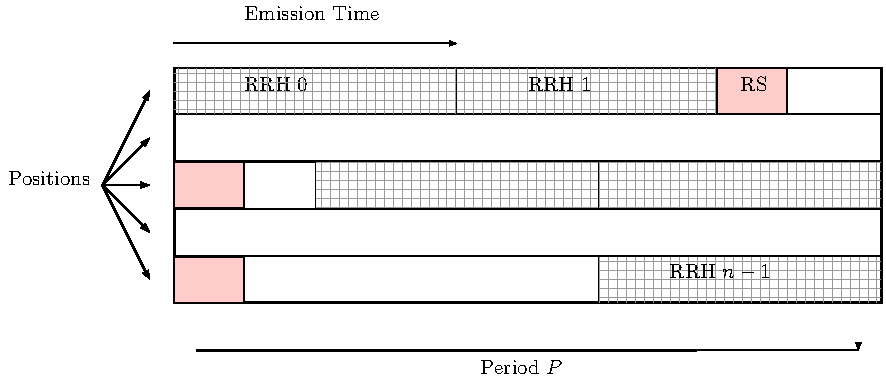
\includegraphics[scale=0.7]{optimalgo.pdf}
     \caption{Organization of the bunches with the balancing algorithm.}   \label{fig:optimalgo}
  \end{figure}
  
  We want to observe the impact of this algorithm on BE traffic. Since our previous parameters did not allow several RRH to share a frequency, we now set $ET = 200$, that correspond to a C-RAN flow of $2$Gbps. This is not out of context since the exact split (the C-RAN split is the degree of centralization of the computation units in the cloud) of the C-RAN is not fully determined yet~\cite{REF}.\todo {la ref} To keep a load similar to the load in the previous experiment, we set the number of antennas to $n=12$. The others parameters are all the one described in the sec~\ref{sec:parameters}.
  The following experiment shows us the impact of the balancing algorithm on the BE traffics. We chose to compare those results to a simulation with the same parameters but with the full opportunistic method of sec~\ref{sec:cranprio}.
  
   \begin{figure}[h]
\centering
      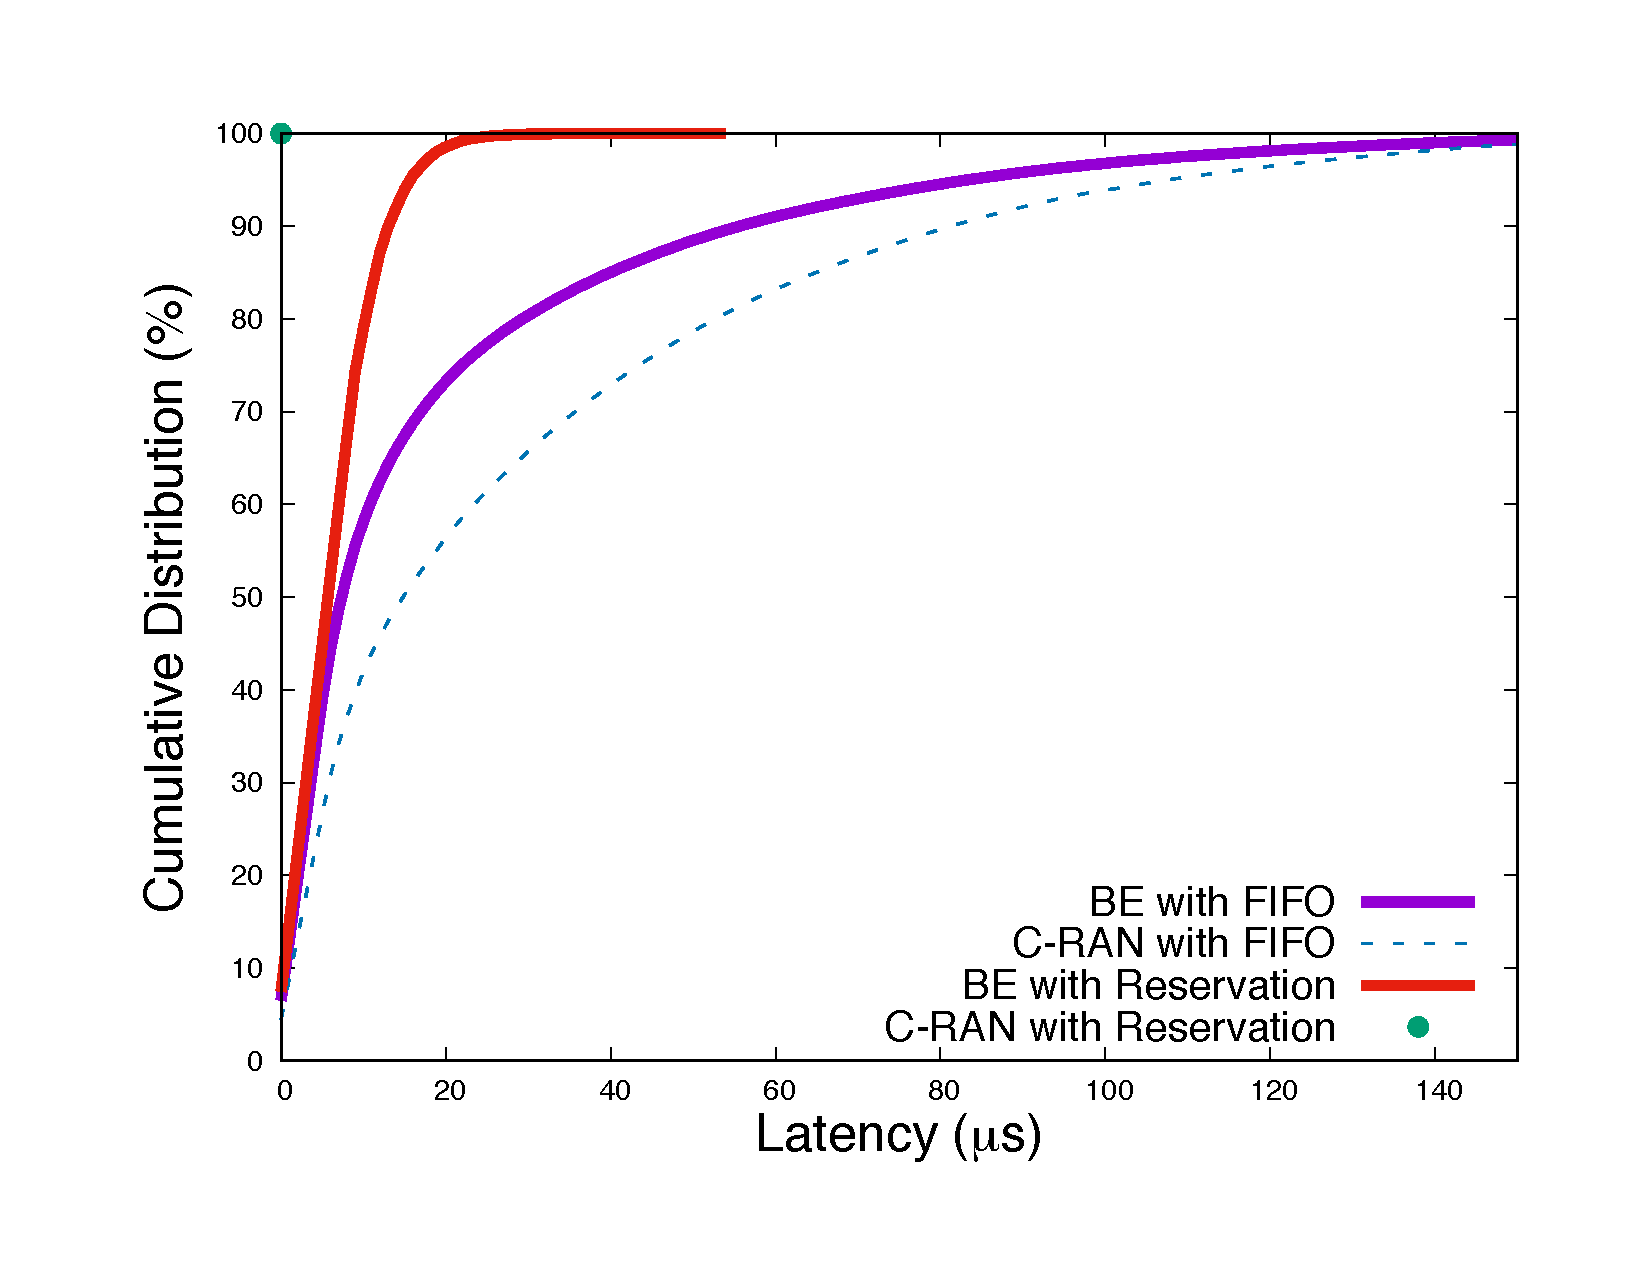
\includegraphics[scale=0.4]{optim.pdf}
     \caption{Balancing algorithm performance on the N-GREEN optical ring.}   \label{fig:optimres}
  \end{figure}
  
  As fig~\ref{fig:optimres} shows, the full repartition algorithm ensures a lower sojourn time to BE PDUs than the full opportunistic method, which gave the best result for the BE traffic. Indeed, since we remove the random aspect of the C-RAN PDUs generation, we balanced the load over the period an then increased the BE performances while we totally removed the C-RAN PDUs sojourn time.
  
  \bibliographystyle{ieeetr}
\bibliography{src}

\end{document}